\documentclass[10pt, a4paper, landscape, xcolor=dvipsnames]{extarticle}
\pagestyle{empty} % Keine Seitennummern

% Verwendete Pakete

	\usepackage[utf8]{inputenc}
	\usepackage[top=0.7cm, bottom=0.9cm, left=0.65 cm, right=0.65 cm, ]{geometry}
	\usepackage{amsmath}
	\usepackage{amsfonts}
	\usepackage{lmodern}
	\usepackage{graphicx}
	\setlength{\parindent}{0pt}
	\usepackage[normalem]{ulem}
	\usepackage[dvipsnames]{xcolor}
	\usepackage{enumitem}
	\usepackage{mathabx}
	\usepackage{enumitem}
	\usepackage{colortbl}
	\usepackage[ngerman]{babel}
	\usepackage{mathtools}
	\usepackage{wallpaper}
	\usepackage{changepage}
	\usepackage{tikz}
	\usepackage{tabularx}
	\usepackage{tcolorbox}
	\usepackage{lipsum}
	\usepackage{multicol}
	\usepackage{letltxmacro}
	\usepackage{tabularx}
	\usepackage{multicol}
	\usepackage{multicol}
	\usepackage{calc}
	\usepackage{ifthen}
	\usepackage{hyperref}
	\usepackage{graphicx}
	\graphicspath{ {./img/} }
	\usepackage{wrapfig}


% Spalteneinstellungen

	\setlength\columnsep{3mm}
	\setlength{\columnseprule}{0pt}
	
% Neue Befehle

	% Bullet-Symbol für Aufzählungen
	\renewcommand\textbullet{\ensuremath{\bullet}}
	
	% Eingekreiste Nummern für Aufzählungen
	\newcommand*\circled[1]{\tikz[baseline=(char.base)]{
            \node[shape=circle,draw,inner sep=1.2pt] (char) {#1};}}
            
    % Horizontale Punkte
    \LetLtxMacro\orgddots\ddots
    \makeatletter
	\DeclareRobustCommand\vdots{%
	  \mathpalette\@vdots{}%
	}
	\newcommand*{\@vdots}[2]{%
	  % #1: math style
	  % #2: unused
	  \sbox0{$#1\cdotp\cdotp\cdotp\m@th$}%
	  \sbox2{$#1.\m@th$}%
	  \vbox{%
	    \dimen@=\wd0 %
	    \advance\dimen@ -3\ht2 %
	    \kern.5\dimen@
	    % remove side bearings
	    \dimen@=\wd2 %
	    \advance\dimen@ -\ht2 %
	    \dimen2=\wd0 %
	    \advance\dimen2 -\dimen@
	    \vbox to \dimen2{%
	      \offinterlineskip
	      \copy2 \vfill\copy2 \vfill\copy2 %
	    }%
	   }%
	}
	\DeclareRobustCommand\ddots{%
		\mathinner{%
		   \mathpalette\@ddots{}%
		   \mkern\thinmuskip
		}%
	}
	
	% Vertikale Punkte
	\DeclareRobustCommand\ddots{%
		  \mathinner{%
		    \mathpalette\@ddots{}%
		    \mkern\thinmuskip
		  }%
		}
		\newcommand*{\@ddots}[2]{%
		  % #1: math style
		  % #2: unused
		  \sbox0{$#1\cdotp\cdotp\cdotp\m@th$}%
		  \sbox2{$#1.\m@th$}%
		  \vbox{%
		    \dimen@=\wd0 %
		    \advance\dimen@ -3\ht2 %
		    \kern.5\dimen@
		    % remove side bearings
		    \dimen@=\wd2 %
		    \advance\dimen@ -\ht2 %
		    \dimen2=\wd0 %
		    \advance\dimen2 -\dimen@
		    \vbox to \dimen2{%
		      \offinterlineskip
		      \hbox{$#1\mathpunct{.}\m@th$}%
		      \vfill
		      \hbox{$#1\mathpunct{\kern\wd2}\mathpunct{.}\m@th$}%
		      \vfill
		      \hbox{$#1\mathpunct{\kern\wd2}\mathpunct{\kern\wd2}\mathpunct{.}\m@th$}%
		    }%
		  }%
		}
	\makeatother
	
	% Schriftart
	\renewcommand{\familydefault}{\sfdefault}
	
	% Dokument-Info Block	
	\newcommand{\DocumentInfo}[3]{
	\begin{tcolorbox}[
			arc=0mm, 
			colback = white!38!black,
			boxrule=0pt,
			toptitle=1mm,
			bottomtitle=1mm,
			right=2mm,
			left=2mm,
			leftright skip = -0.5mm,
			title= \huge \center \textbf{#1} \par \large \vskip1mm #2 \par \vskip1mm \small 	Version: \today,
			fontupper=\color{white},
			after skip = 0 mm,
			top=0.1mm,
			bottom=1mm]
		
		\small #3
	\vskip1mm	
	\end{tcolorbox}
	}
	
	% Überschrift
	\renewcommand{\section}[1]{
	\begin{tcolorbox}[
			arc=0mm,
			colback=white!38!black,
			colframe=white,
			bottomrule = 0 mm,
			toprule = 0 mm,
			leftrule = 0 mm,
			rightrule = 0 mm,
			valign=center,
			left=0.5mm,
			top= 0.7 mm,
			bottom= 0.7 mm,
			fontupper=\color{white},
			before skip = 0mm,
			leftright skip = -0.5mm,
			after skip = 0 mm]

		\textbf{#1}
	\end{tcolorbox}
	}
	
	% Abschnitt	
	\renewcommand{\subsection}[2]{
	\begin{tcolorbox}[
			arc=0mm,
			colback=white!75!black,
			colframe=white,
			bottomrule = 0 mm,
			toprule = 0 mm,
			leftrule = 0 mm,
			rightrule = 0 mm,
			valign=center,
			left=0.5mm,
			top=0.2mm,
			bottom=0.2mm,
			before skip = 0mm,
			leftright skip = -0.5mm,
			after skip = 1.4 mm]
			
		\small \textbf{#1}
	\end{tcolorbox}
	
	\begin{adjustwidth}{0.5mm}{1mm}
		\small
		#2
		\vspace{0.5mm}
	\end{adjustwidth}
	}
	
	% Weisser Balken zwischen Abschnitten
	\newcommand{\WhiteSpace}[0]{
	\begin{tcolorbox}[
			arc=0mm,
			colback=white,
			colframe=white,
			bottomrule = 0 mm,
			toprule = 0 mm,
			leftrule = 0 mm,
			rightrule = 0 mm,
			valign=center,
			left=0.5mm,
			top= -0.2 mm,
			bottom= -0.2 mm,
			fontupper=\color{white},
			before skip = 0mm,
			leftright skip = -0.5mm,
			after skip = 0 mm]
	
	\end{tcolorbox}
	}
	
% Hintergrundbild (graue Spalten)

%	\CenterWallPaper{1}{0_Setup/background.pdf}

% TabularX Zeug (Paket für Tabellen)

	\newcolumntype{C}[1]{>{\centering\arraybackslash}p{#1}}

% TikZ Zeug (Paket für Vektorgraphiken)

	\usetikzlibrary{decorations.pathreplacing,calc}

	\newcommand{\tikzmark}[2][-3pt]{\tikz[remember picture, overlay, baseline=-0.5ex]\node[#1](#2){};}
	
	\tikzset{brace/.style={decorate, decoration={brace}},
	 brace mirrored/.style={decorate, decoration={brace,mirror}},
	}
	
	\newcounter{brace}
	\setcounter{brace}{0}
	\newcommand{\drawbrace}[3][brace]{%
	 \refstepcounter{brace}
	 \tikz[remember picture, overlay]\draw[#1] (#2.center)--(#3.center)node[pos=0.5, name=brace-\thebrace]{};
	}
	
	\newcommand{\annote}[3][]{%
	 \tikz[remember picture, overlay]\node[#1] at (#2) {#3};
	}

\begin{document}

% Vier Spalten
\begin{multicols*}{3}

% Info über das Dokument
\DocumentInfo
{Analysis 2 S2} %Titel
{Raphael Nambiar} %Untertitel

\WhiteSpace

% Dokumentinhalt
\section{Integrieren}

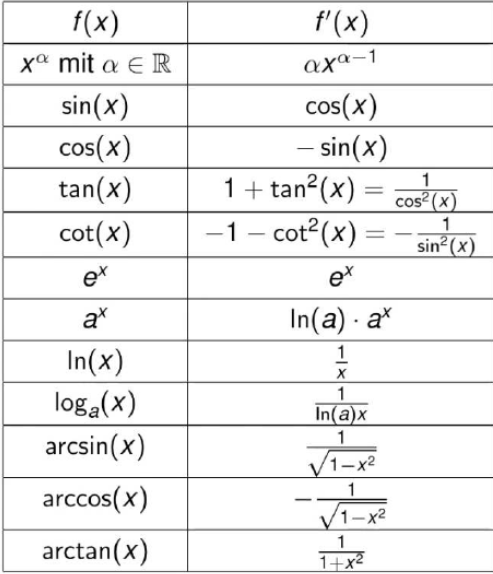
\includegraphics[scale=0.35]{ableitungen.png} 
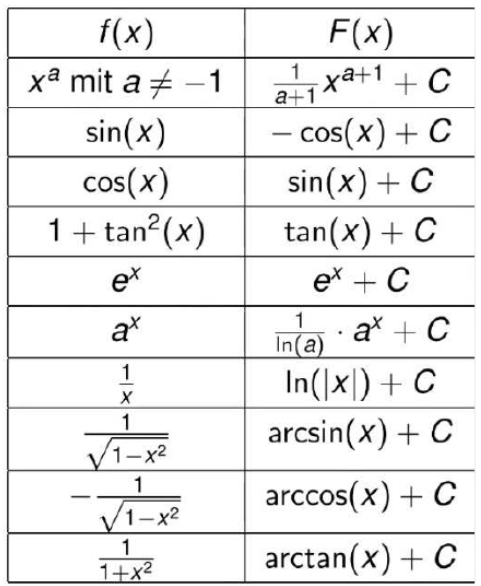
\includegraphics[scale=0.35]{stammfunktionen.png} 

\subsection{Integration durch Substitution}
{\circled{1} Substitutionsgleichung für $x: u = g(x)$}

{\circled{2} Substitutionsgleichung für $dx:$}

$ \frac{du}{dx} = g'(x)_{\tiny(Ableitung)} \to dx = \frac{du}{g'(x)}$

{\circled{3} Integralsubstitution: Einsetzen von $ u $ und $ dx $ aus 1. und 2 in Ursprung}

{\circled{4} Integration von 3.}

{\circled{5} Rücksubstitution (nur unbestimmte Integrale)}


\begin{multicols}{2}
{Beispiel:}

 
\columnbreak

{\circled{1} $ u = 2x $}
  
{\circled{2} $ dx = \frac{du}{2} $}  

{\circled{3} $ \int_{}{}e^u \cdot  \frac{du}{2} $}

\end{multicols}
\vspace{-10pt}
 {\circled{4} $ \int_{}{}e^u \cdot  \frac{1}{2}du = \frac{1}{2} \cdot  \int_{}{}e^u du \rightarrow \frac{1}{2} e^u + C   $}


{\circled{5} $\frac{1}{2} e^u + C \rightarrow \frac{1}{2} e^{2x} + C$ }



\subsection{Partielle Integration}
{\large $$u(x)\cdot v(x) - \int_{}^{}u'(x) \cdot v(x) \hspace{2px}  dx$$}

\begin{multicols}{2}
{Beispiel:}
 \[ \int_{}{}x\cdot e^x\]
$$ \int_{}{}x\cdot e^x = x\cdot e^x -  \int_{}{}\cdot e^x dx = x\cdot e^x - e^x + C $$
\columnbreak
 
{$u(x)=x$; $v'(x)=e^x$}

{$u'(x)=1$; $v(x)=e^x$}

\end{multicols}





\subsection{Integration durch Partialbruchzerlegung}
{TBD}

\section{Differentialgleichungen (DGL)}
\subsection{Begriffe}
{\textbf{Ordnung:} Ordnung = höchste Ableitung in der DGL}
{\textbf{Linearität:} Funktion und Ableitung sind linear $\rightarrow x^1$ }

\subsection{Separierbare Differentialgleichungen}
{Eine Differentialgleichung 1. Ordnung heisst separierbar wenn:}
$$ y' = f(x)\cdot g(x)$$

{How To:}

\circled{1} $y' = \frac{dy}{dx} = f(x)\cdot g(y) $

\circled{2} {Trennung der Variablen:} $\frac{dy}{g(y)} = f(x)\cdot dx$

\circled{3} {Integration auf beiden Seiten der Gleichung (if possible):} $$\int_{}^{}{\frac{dy}{g(y)}=\int_{}^{}f(x)dx}$$
\circled{4} {Auflösen nach y (falls möglich!)}

\begin{multicols}{2}
{Beispiel:}

$$y' = y^2 = sin(x)$$

\circled{1} $y' = \frac{dy}{dx}=\frac{sin(x)}{y^2}$

\circled{2} $y^2\cdot dy = sin(x)\cdot dx $
\columnbreak
 
\circled{3} 

\circled{4} 

\end{multicols}



\subsection{Autonome Differentialgleichungen}


\WhiteSpace

\mbox{}
	
\end{multicols*} 

\end{document}
